% Options for packages loaded elsewhere
\PassOptionsToPackage{unicode}{hyperref}
\PassOptionsToPackage{hyphens}{url}
\PassOptionsToPackage{dvipsnames,svgnames,x11names}{xcolor}
%
\documentclass[
]{article}

\usepackage{amsmath,amssymb}
\usepackage{iftex}
\ifPDFTeX
  \usepackage[T1]{fontenc}
  \usepackage[utf8]{inputenc}
  \usepackage{textcomp} % provide euro and other symbols
\else % if luatex or xetex
  \usepackage{unicode-math}
  \defaultfontfeatures{Scale=MatchLowercase}
  \defaultfontfeatures[\rmfamily]{Ligatures=TeX,Scale=1}
\fi
\usepackage[sfdefault]{Roboto}
\ifPDFTeX\else  
    % xetex/luatex font selection
\fi
% Use upquote if available, for straight quotes in verbatim environments
\IfFileExists{upquote.sty}{\usepackage{upquote}}{}
\IfFileExists{microtype.sty}{% use microtype if available
  \usepackage[]{microtype}
  \UseMicrotypeSet[protrusion]{basicmath} % disable protrusion for tt fonts
}{}
\usepackage{xcolor}
\usepackage[top=10pc,bottom=10pc,left=11pc,right=11pc,heightrounded]{geometry}
\setlength{\emergencystretch}{3em} % prevent overfull lines
\setcounter{secnumdepth}{-\maxdimen} % remove section numbering


\providecommand{\tightlist}{%
  \setlength{\itemsep}{0pt}\setlength{\parskip}{0pt}}\usepackage{longtable,booktabs,array}
\usepackage{calc} % for calculating minipage widths
% Correct order of tables after \paragraph or \subparagraph
\usepackage{etoolbox}
\makeatletter
\patchcmd\longtable{\par}{\if@noskipsec\mbox{}\fi\par}{}{}
\makeatother
% Allow footnotes in longtable head/foot
\IfFileExists{footnotehyper.sty}{\usepackage{footnotehyper}}{\usepackage{footnote}}
\makesavenoteenv{longtable}
\usepackage{graphicx}
\makeatletter
\def\maxwidth{\ifdim\Gin@nat@width>\linewidth\linewidth\else\Gin@nat@width\fi}
\def\maxheight{\ifdim\Gin@nat@height>\textheight\textheight\else\Gin@nat@height\fi}
\makeatother
% Scale images if necessary, so that they will not overflow the page
% margins by default, and it is still possible to overwrite the defaults
% using explicit options in \includegraphics[width, height, ...]{}
\setkeys{Gin}{width=\maxwidth,height=\maxheight,keepaspectratio}
% Set default figure placement to htbp
\makeatletter
\def\fps@figure{htbp}
\makeatother

% -----------------------
% CUSTOM PREAMBLE STUFF
% -----------------------

% -----------------
% Typography tweaks
% -----------------
% Indent size
\setlength{\parindent}{1pc}  % 1p0

% Fix widows and orphans
\usepackage[all,defaultlines=2]{nowidow}

% List things
\usepackage{enumitem}
% Same document-level indentation for ordered and ordered lists
\setlist[1]{labelindent=\parindent}
\setlist[itemize]{leftmargin=*}
\setlist[enumerate]{leftmargin=*}

% Wrap definition list terms
% https://tex.stackexchange.com/a/9763/11851
\setlist[description]{style=unboxed}


% For better TOCs
\usepackage{tocloft}

% Remove left margin in lists inside longtables
% https://tex.stackexchange.com/a/378190/11851
\AtBeginEnvironment{longtable}{\setlist[itemize]{nosep, wide=0pt, leftmargin=*, before=\vspace*{-\baselineskip}, after=\vspace*{-\baselineskip}}}


% -----------------
% Title block stuff
% -----------------

% Abstract
\usepackage[overload]{textcase}
\usepackage[runin]{abstract}
\renewcommand{\abstractnamefont}{\sffamily\footnotesize\bfseries\MakeUppercase}
\renewcommand{\abstracttextfont}{\sffamily\small}
\setlength{\absleftindent}{\parindent * 2}
\setlength{\absrightindent}{\parindent * 2}
\abslabeldelim{\quad}
\setlength{\abstitleskip}{-\parindent}


% Keywords
\newenvironment{keywords}
{\vskip -3em \hspace{\parindent}\small\sffamily{\sffamily\footnotesize\bfseries\MakeUppercase{Keywords}}\quad}
{\vskip 3em}

  
% Title
\usepackage{titling}
\setlength{\droptitle}{3em}
\pretitle{\par\vskip 5em \begin{flushleft}\LARGE\sffamily\bfseries}
\posttitle{\par\end{flushleft}\vskip 0.75em}


% Authors
%
% PHEW this is complicated for a number of reasons!
%
% When using \and with multiple authors, the article class in LaTeX wraps each 
% author block in a tabluar environment with a hardcoded center alignment. It's 
% possible to use \preauthor{} to start tabulars with a left alignment {l}, but 
% that only applies to the first author because the others all use \and with the 
% hardcoded {c}. But we can override the \and command and add our own {l}
%
% (See https://github.com/rstudio/rmarkdown/issues/1716#issuecomment-560601691 
% for an example of redefining \and to just be \\)
%
% That's all great, except tabulars have some amount of default horizontal 
% padding, which makes left-aligned author blocks not actuall get fully 
% left-aligned on the page. We can set the horizontal padding for the column to 
% 0, but it requires some wonky syntax: {@{\hspace{0em}}l@{}}
\renewcommand{\and}{\end{tabular} \hskip 3em \begin{tabular}[t]{@{\hspace{0em}}l@{}}}
\preauthor{\begin{flushleft}
           \lineskip 1.5em 
           \begin{tabular}[t]{@{\hspace{0em}}l@{}}}
\postauthor{\end{tabular}\par\end{flushleft}}

% Omit the date since the \published command does that
\predate{}
\postdate{}

% Command for a note at the top of the first page describing the publication
% status of the paper.
\newcommand{\published}[1]{%
   \gdef\puB{#1}}
   \newcommand{\puB}{}
   \renewcommand{\maketitlehooka}{%
       \par\noindent\footnotesize\sffamily \puB}


% ------------------
% Section headings
% ------------------
\usepackage{titlesec}
\titleformat*{\section}{\Large\sffamily\bfseries\raggedright}
\titleformat*{\subsection}{\large\sffamily\bfseries\raggedright}
\titleformat*{\subsubsection}{\normalsize\sffamily\bfseries\raggedright}
\titleformat*{\paragraph}{\small\sffamily\bfseries\raggedright}

% \titlespacing{<command>}{<left>}{<before-sep>}{<after-sep>}
% Starred version removes indentation in following paragraph
\titlespacing*{\section}{0em}{2em}{0.1em}
\titlespacing*{\subsection}{0em}{1.25em}{0.1em}
\titlespacing*{\subsubsection}{0em}{0.75em}{0em}


% -----------
% Footnotes
% -----------
% NB: footmisc has to come after biblatex because of conflicts
\usepackage[bottom, flushmargin]{footmisc}
\renewcommand*{\footnotelayout}{\footnotesize}

\addtolength{\skip\footins}{10pt}    % vertical space between rule and main text
\setlength{\footnotesep}{5pt}  % vertical space between footnotes


% ----------
% Captions
% ----------
\usepackage[font={small,sf}, labelfont={small,sf,bf}]{caption}


% --------
% Macros
% --------
% pandoc will not convert text within \begin{} XXX \end{} to Markdown and will
% treat it as regular TeX. Because of this, it's impossible to do stuff like
% this:

% \begin{landscape}
%
% | One | Two   |
% |-----+-------|
% | my  | table |
% | is  | nice  |
%
% \end{landscape}
%
% Since it'll render like: | One | Two | |—–+——-| | my | table | | is | nice |
% 
% BUT, from this http://stackoverflow.com/a/41945462/120898 we can get around
% this by creating new commands for \begin and \end, like this:
\newcommand{\blandscape}{\begin{landscape}}
\newcommand{\elandscape}{\end{landscape}}

% \blandscape
%
% | One | Two   |
% |-----+-------|
% | my  | table |
% | is  | nice  |
%
% \elandscape

% Same thing, but for generic groups
% But can't use \bgroup and \egroup because those are built-in TeX things
\newcommand{\stgroup}{\begingroup}
\newcommand{\fingroup}{\endgroup}


% ---------------------------
% END CUSTOM PREAMBLE STUFF
% ---------------------------
\usepackage{float}
\usepackage{tabularray}
\usepackage[normalem]{ulem}
\usepackage{graphicx}
\UseTblrLibrary{booktabs}
\UseTblrLibrary{siunitx}
\NewTableCommand{\tinytableDefineColor}[3]{\definecolor{#1}{#2}{#3}}
\newcommand{\tinytableTabularrayUnderline}[1]{\underline{#1}}
\newcommand{\tinytableTabularrayStrikeout}[1]{\sout{#1}}
\usepackage{pdflscape}
\UseTblrLibrary{varwidth, counter}
\renewcommand{\thetable}{S\arabic{table}}
\renewcommand{\thefigure}{S\arabic{figure}}
\makeatletter
\@ifpackageloaded{caption}{}{\usepackage{caption}}
\AtBeginDocument{%
\ifdefined\contentsname
  \renewcommand*\contentsname{Table of contents}
\else
  \newcommand\contentsname{Table of contents}
\fi
\ifdefined\listfigurename
  \renewcommand*\listfigurename{List of Figures}
\else
  \newcommand\listfigurename{List of Figures}
\fi
\ifdefined\listtablename
  \renewcommand*\listtablename{List of Tables}
\else
  \newcommand\listtablename{List of Tables}
\fi
\ifdefined\figurename
  \renewcommand*\figurename{Figure}
\else
  \newcommand\figurename{Figure}
\fi
\ifdefined\tablename
  \renewcommand*\tablename{Table}
\else
  \newcommand\tablename{Table}
\fi
}
\@ifpackageloaded{float}{}{\usepackage{float}}
\floatstyle{ruled}
\@ifundefined{c@chapter}{\newfloat{codelisting}{h}{lop}}{\newfloat{codelisting}{h}{lop}[chapter]}
\floatname{codelisting}{Listing}
\newcommand*\listoflistings{\listof{codelisting}{List of Listings}}
\makeatother
\makeatletter
\makeatother
\makeatletter
\@ifpackageloaded{caption}{}{\usepackage{caption}}
\@ifpackageloaded{subcaption}{}{\usepackage{subcaption}}
\makeatother
\ifLuaTeX
  \usepackage{selnolig}  % disable illegal ligatures
\fi
\usepackage{bookmark}

\IfFileExists{xurl.sty}{\usepackage{xurl}}{} % add URL line breaks if available
\urlstyle{same} % disable monospaced font for URLs
\hypersetup{
  pdftitle={Perceptions of drinking water management and safety: A public survey of U.S. residents},
  pdfauthor={Michael Schramm; Allen Berthold; Audrey McCrary; Stephanie deVilleneuve},
  colorlinks=true,
  linkcolor={DarkSlateBlue},
  filecolor={Maroon},
  citecolor={DarkSlateBlue},
  urlcolor={DarkSlateBlue},
  pdfcreator={LaTeX via pandoc}}

% -----------------------
% END-OF-PREAMBLE STUFF
% -----------------------


% ----------
% BibLaTeX
% ----------
\usepackage[style=apa,backend=biber]{biblatex}

\setlength\bibitemsep{0pt}  % No space between bib entries
\renewcommand*{\bibfont}{\footnotesize}  % Use smaller font
\setlength\bibhang{\parindent}  % Match document indentation

% Fix biblatex's odd preference for using In: by default.
\renewbibmacro{in:}{%
  \ifentrytype{article}{}{%
  \printtext{\bibstring{}\intitlepunct}}}

\addbibresource{}

% ---------------------- 
% Title block elements
% ---------------------- 
\usepackage{orcidlink}  % Create automatic ORCID icons/links

\title{Perceptions of drinking water management and safety: A public
survey of U.S. residents}

\usepackage{etoolbox}
\makeatletter
\providecommand{\subtitle}[1]{% add subtitle to \maketitle
  \apptocmd{\@title}{\par {\vskip 0.25em \large #1 \par}}{}{}
}
\makeatother
\subtitle{Supplementary Materials}

\author{
{\large Michael Schramm~\orcidlink{0000-0003-1876-6592}}%
 \\%
Texas A\&M AgriLife \\%
{\footnotesize \url{michael.schramm@ag.tamu.edu}} \and
{\large Allen Berthold}%
 \\%
Texas A\&M AgriLife \\%
{\footnotesize \url{}} \and
{\large Audrey McCrary~\orcidlink{0000-0002-7061-6113}}%
 \\%
Texas A\&M AgriLife \\%
{\footnotesize \url{}} \and
{\large Stephanie deVilleneuve~\orcidlink{0009-0002-3984-035X}}%
 \\%
Texas A\&M AgriLife \\%
{\footnotesize \url{}} \and
}

\date{}


% Typeset URLs in the same font as their parent environment
%
% This has to come at the end of the preamble, after any biblatex stuff because 
% some biblatex styles (like APA) define their own \urlstyle{}
\usepackage{url}
\urlstyle{same}

% ---------------------------
% END END-OF-PREAMBLE STUFF
% ---------------------------
\begin{document}
% ---------------
% TITLE SECTION
% ---------------
\published{\textbf{}}

\maketitle



% -------------------
% END TITLE SECTION
% -------------------


\begin{longtblr}[         %% tabularray outer open
caption={},
entry=none,label=none,
note{1}={Matrix style question.},
label=tblr:quest,
caption={Survey questions.},
]                     %% tabularray outer close
{                     %% tabularray inner open
colspec={Q[]Q[]},
measure=vbox, stretch=-1, column{1}={wd=75mm}, column{2}={wd=70mm}, hline{3-7}={dashed},
}                     %% tabularray inner close
\toprule
Questions & Response Options \\ \midrule %% TinyTableHeader
What is the source of your household tap water?                                                                                                                                                                                                                                                                                                                                                                                                                              & \begin{itemize}[nosep]    \item[$\square$] Public supply - municipal     \item[$\square$] Public supply - rural water district    \item[$\square$] Private supply - private well, river, pond, lake    \item[$\square$] Private supply - rainwater harvest system    \item[$\square$] I don't know    \item[$\square$] Other    \end{itemize}                                                                                                                                                                                                                                                                            \\
What is your main source of drinking water?                                                                                                                                                                                                                                                                                                                                                                                                                                  & \begin{itemize}[nosep]    \item[$\square$] Unfiltered tap water    \item[$\square$] Filtered tap water    \item[$\square$] Bottled or prepackaged water    \item[$\square$] Other    \end{itemize}                                                                                                                                                                                                                                                                                                                                                                                                                               \\
Has your primary source of drinking water ever been impacted by any of the following issues? (select all that apply)                                                                                                                                                                                                                                                                                                                                                         & \begin{itemize}[nosep]    \item[$\square$] Odd taste    \item[$\square$] Odd smell    \item[$\square$] Discolored water    \item[$\square$] Cloudy water    \item[$\square$] Staining of clothes, teeth, or skin    \item[$\square$] Saltiness (high salt content)    \item[$\square$] Hardness or scale buildup (high mineral content)    \item[$\square$] Corrosion of pipes or water fixtures    \item[$\square$] Boil water notice    \item[$\square$] Water shortage    \item[$\square$] None of the above    \item[$\square$] Other    \end{itemize}                                       \\
To your knowledge, has your primary source of drinking water been impacted by any of the following contaminants? (select all that apply)                                                                                                                                                                                                                                                                                                                                     & \begin{itemize}[nosep]    \item[$\square$] Disinfection byproducts (DFBs)    \item[$\square$] Fertilizers (nitrates, phosphates)    \item[$\square$] Heavy metals (lead, arsenic, mercury, etc.)    \item[$\square$] Industrial chemicals    \item[$\square$] Microplastics    \item[$\square$] PFAS (per- and polyfluoroalkyl substances)    \item[$\square$] Pathogens (bacteria, viruses, amoebas)    \item[$\square$] Pesticides    \item[$\square$] Petroleum products    \item[$\square$] Pharmaceuticals    \item[$\square$] None of the above    \item[$\square$] Other    \end{itemize} \\
On a scale from 0 to 10, how safe do you believe your drinking water is for consumption?                                                                                                                                                                                                                                                                                                                                                                                     & Scale, 0-10                                                                                                                                                                                                                                                                                                                                                                                                                                                                                                                                                                                                                                          \\
\textsuperscript{1}What is your level of trust in the following entities for making sure drinking water is safe for consumption:    \begin{itemize}[nosep]    \item Federal government    \item State government    \item Local government    \item Water utility    \item Landlords, property manager    \item Household residents    \end{itemize}                                                                                                & \begin{itemize}[nosep]    \item[$\square$] Do not trust at all    \item[$\square$] Somewhat trust    \item[$\square$] Moderately trust    \item[$\square$] Mostly trust    \item[$\square$] Fully trust    \end{itemize}                                                                                                                                                                                                                                                                                                                                                                                                     \\
\textsuperscript{1}How often do you use the following sources to get information about drinking water quality?    \begin{itemize}[nosep]    \item Local news agency    \item National news agency    \item Local newspaper    \item National newspaper    \item Social media    \item Radio or podcast    \item Word of mouth    \item Email    \item Government agencies    \item My water provider    \item Other    \end{itemize} & \begin{itemize}[nosep]    \item[$\square$] Never    \item[$\square$] Occasionally    \item[$\square$] Sometimes    \item[$\square$] Often    \item[$\square$] Always    \end{itemize}                                                                                                                                                                                                                                                                                                                                                                                                                                        \\
\bottomrule
\end{longtblr}

\begin{longtblr}[         %% tabularray outer open
caption={},
caption={Unweighted and weighted survey demographics.}, label=tblr:one,
]                     %% tabularray outer close
{                     %% tabularray inner open
colspec={Q[]Q[]Q[]Q[]Q[]Q[]},
cell{2}{1}={c=6}{},cell{10}{1}={c=6}{},cell{19}{1}={c=6}{},cell{23}{1}={c=6}{},
cell{3}{1}={preto={\hspace{1em}}},
cell{4}{1}={preto={\hspace{1em}}},
cell{5}{1}={preto={\hspace{1em}}},
cell{6}{1}={preto={\hspace{1em}}},
cell{7}{1}={preto={\hspace{1em}}},
cell{8}{1}={preto={\hspace{1em}}},
cell{9}{1}={preto={\hspace{1em}}},
cell{11}{1}={preto={\hspace{1em}}},
cell{12}{1}={preto={\hspace{1em}}},
cell{13}{1}={preto={\hspace{1em}}},
cell{14}{1}={preto={\hspace{1em}}},
cell{15}{1}={preto={\hspace{1em}}},
cell{16}{1}={preto={\hspace{1em}}},
cell{17}{1}={preto={\hspace{1em}}},
cell{18}{1}={preto={\hspace{1em}}},
cell{20}{1}={preto={\hspace{1em}}},
cell{21}{1}={preto={\hspace{1em}}},
cell{22}{1}={preto={\hspace{1em}}},
cell{24}{1}={preto={\hspace{1em}}},
cell{25}{1}={preto={\hspace{1em}}},
cell{26}{1}={preto={\hspace{1em}}},
cell{27}{1}={preto={\hspace{1em}}},
row{2}={,cmd=\bfseries,},
row{10}={,cmd=\bfseries,},
row{19}={,cmd=\bfseries,},
row{23}={,cmd=\bfseries,},
rulesep={0pt}, rowsep={0pt}, colsep = {.5em}, vspan={default},
}                     %% tabularray inner close
\toprule
Value & \vtop{\hbox{Unweighted}\hbox{(n)}} & \vtop{\hbox{Unweighted}\hbox{(\%)}} & \vtop{\hbox{Target}\hbox{(\%)}} & \vtop{\hbox{Weighted}\hbox{(n)}} & \vtop{\hbox{Weighted}\hbox{(\%)}} \\ \midrule %% TinyTableHeader
Age &&&&& \\
18:24                        & 125 & 11.4 & 11.9 & 130.6 & 11.9 \\
25:34                        & 192 & 17.5 & 17.7 & 195.1 & 17.7 \\
35:44                        & 204 & 18.5 & 16.6 & 183.1 & 16.6 \\
45:54                        & 198 & 18.0 & 16.3 & 179.2 & 16.3 \\
55:64                        & 171 & 15.5 & 16.8 & 184.4 & 16.8 \\
65+                          & 208 & 18.9 & 20.7 & 227.6 & 20.7 \\
No answer                    &   2 &  0.2 &   NA &    NA &   NA \\
Education &&&&& \\
Some high school             &  47 &  4.3 &  7.8 &  85.8 &  7.8 \\
High school graduate or GED  & 418 & 38.0 & 49.4 & 543.7 & 49.4 \\
Associate degree             & 178 & 16.2 &  8.3 &  91.3 &  8.3 \\
Bachelor's degree            & 246 & 22.4 & 19.4 & 213.7 & 19.4 \\
Master's degree              & 132 & 12.0 &  8.3 &  91.3 &  8.3 \\
Doctorate or terminal degree &  28 &  2.5 &  1.3 &  14.7 &  1.3 \\
Other                        &  40 &  3.6 &  5.4 &  59.5 &  5.4 \\
No answer                    &  11 &  1.0 &   NA &    NA &   NA \\
Race/Ethnicity &&&&& \\
White                        & 723 & 65.7 & 62.4 & 686.3 & 62.4 \\
Non-white                    & 373 & 33.9 & 37.6 & 413.7 & 37.6 \\
No answer                    &   4 &  0.4 &   NA &    NA &   NA \\
Sex/Gender &&&&& \\
Male                         & 529 & 48.1 & 49.0 & 539.1 & 49.0 \\
Not Male                     & 569 & 51.7 & 51.0 & 560.9 & 51.0 \\
No answer                    &   2 &  0.2 &   NA &    NA &   NA \\
\bottomrule
\end{longtblr}

\begin{figure}

\centering{

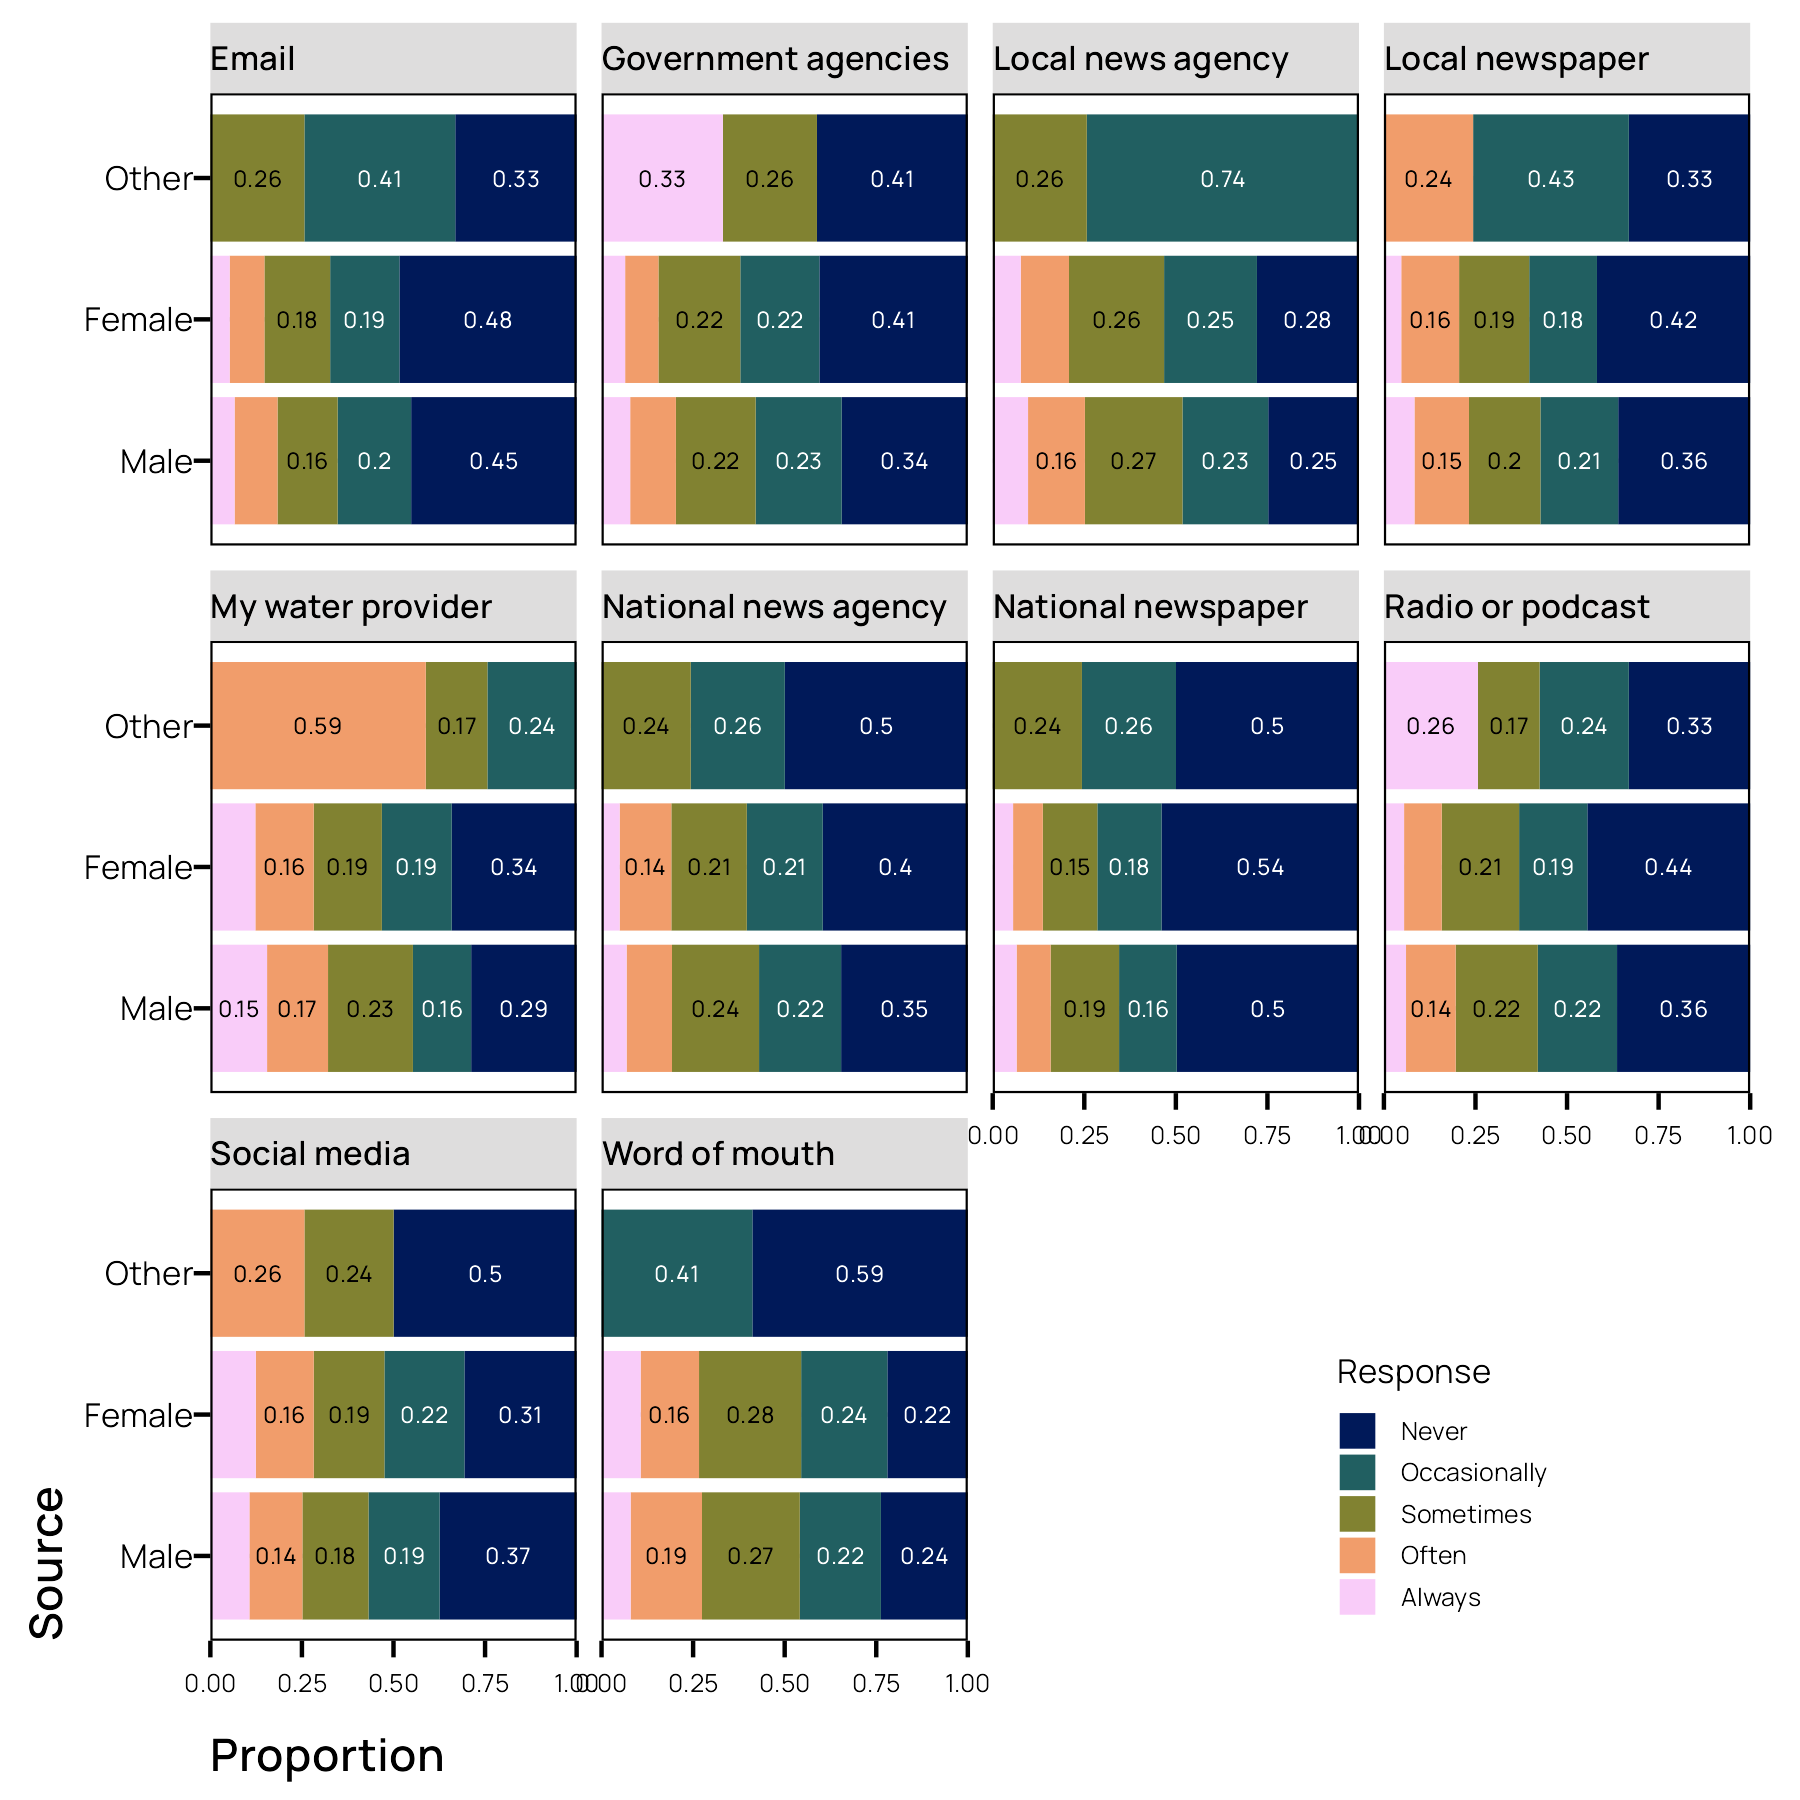
\includegraphics[width=1\textwidth,height=\textheight]{supplementary-materials_files/figure-pdf/fig-news-sex-1.png}

}

\caption{\label{fig-news-sex}Sources of drinking water quality
information by sex/gender.}

\end{figure}%

\begin{figure}

\centering{

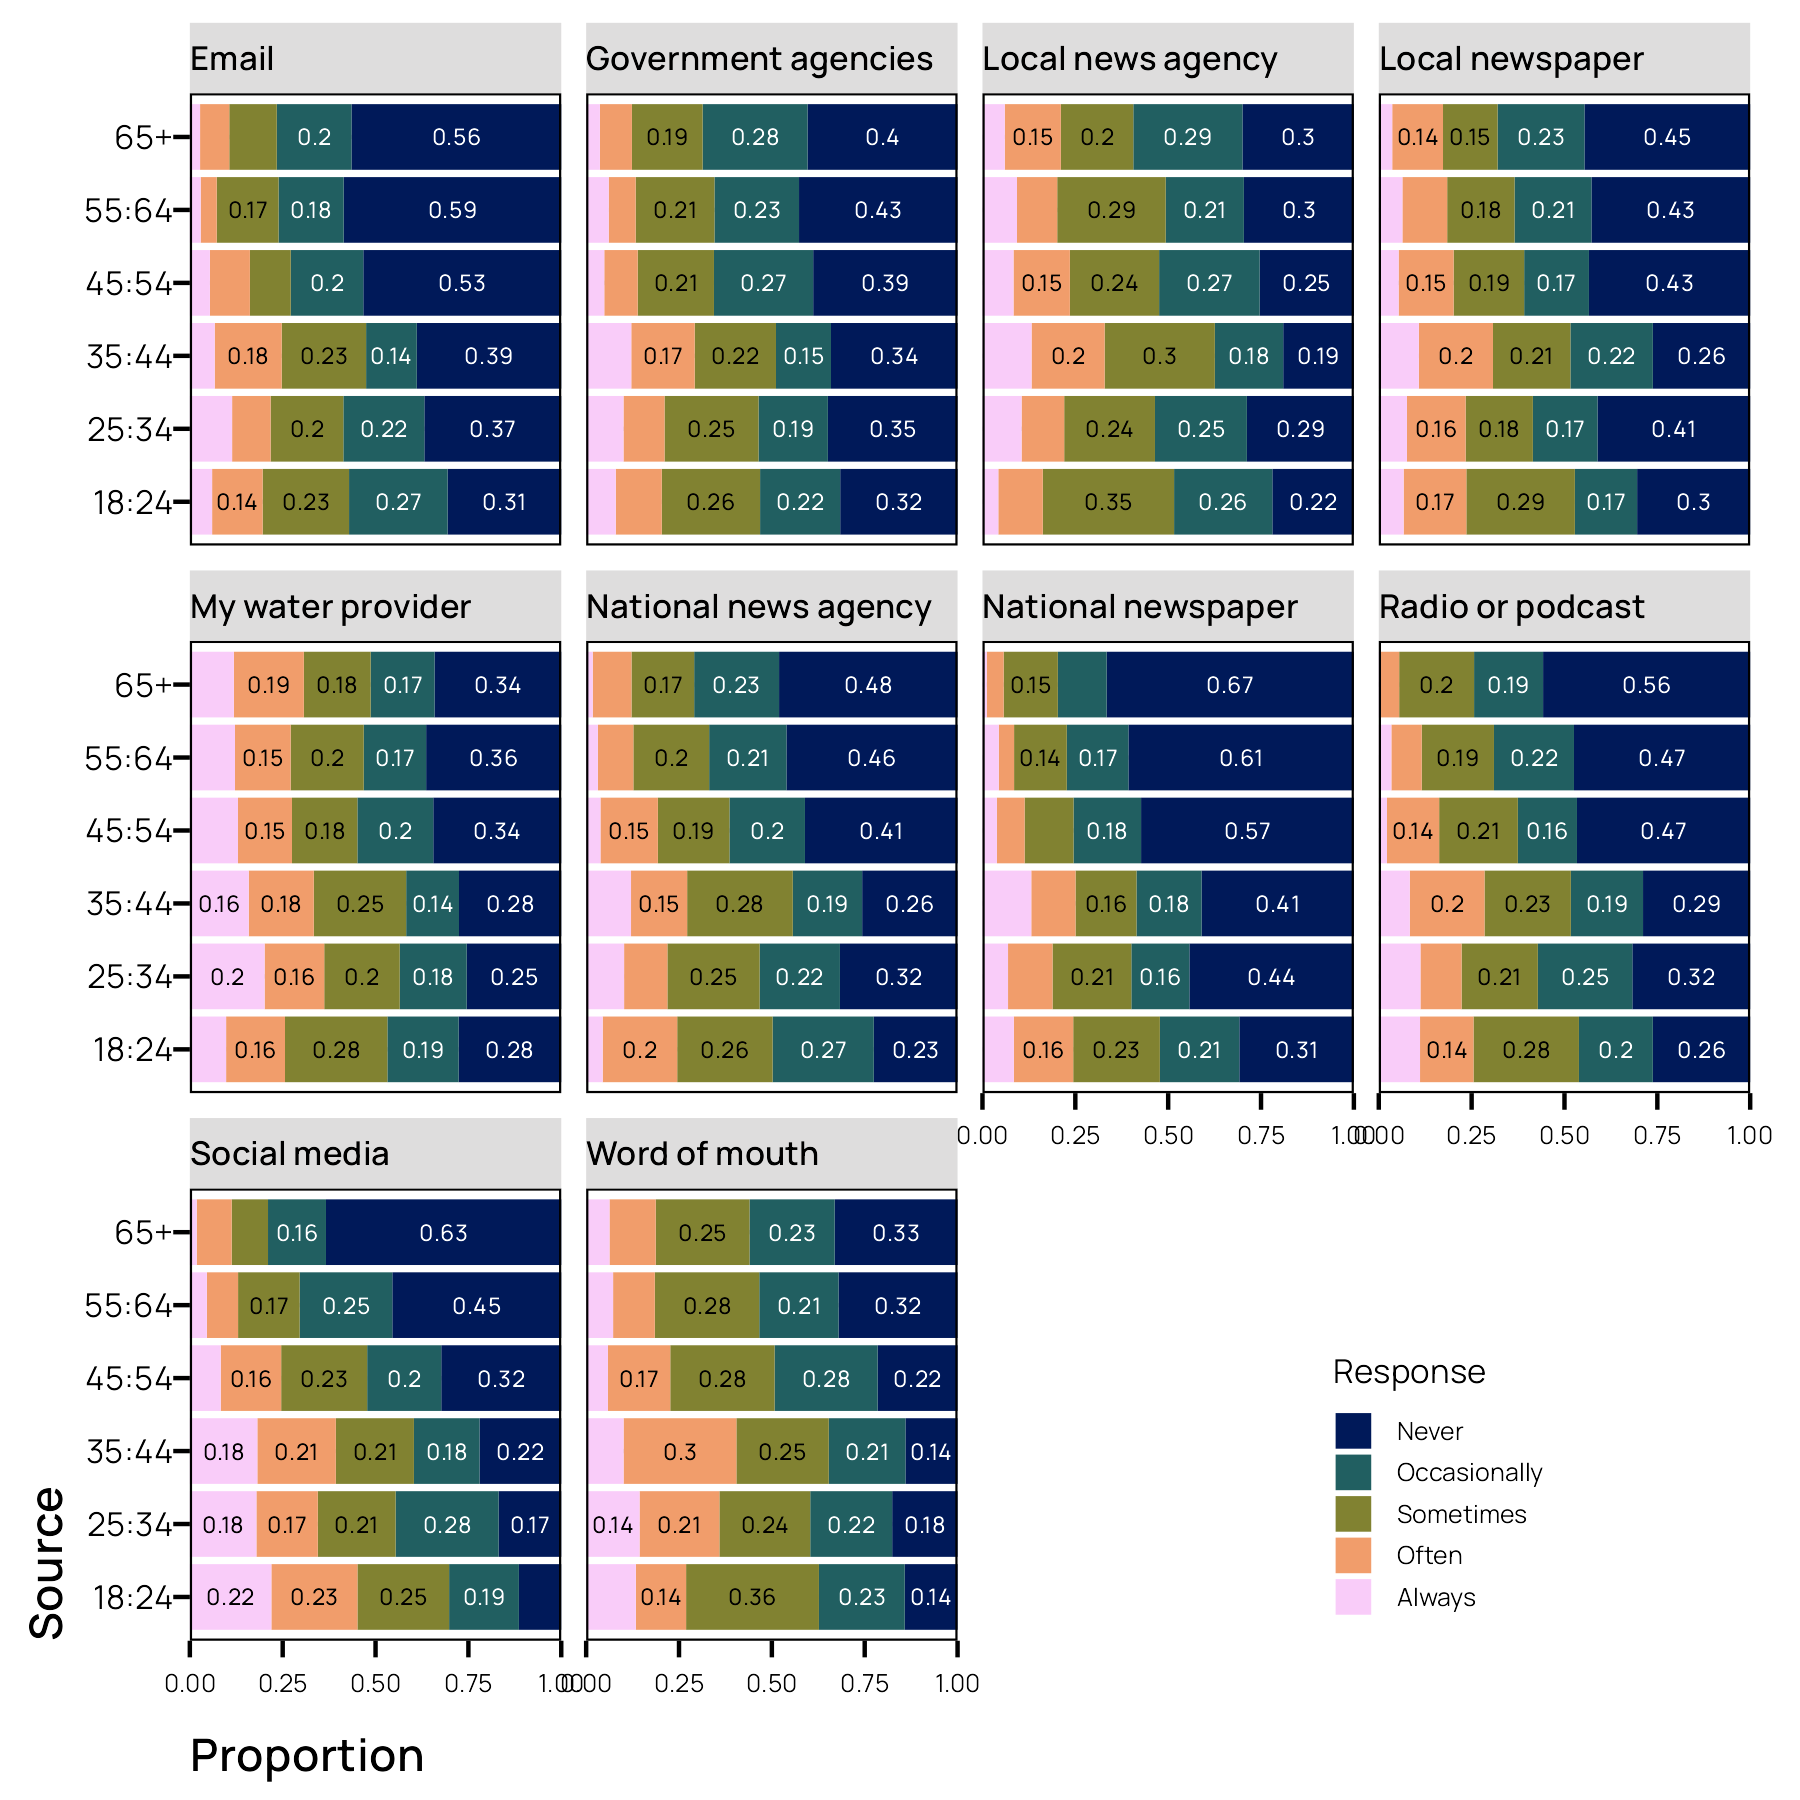
\includegraphics[width=1\textwidth,height=\textheight]{supplementary-materials_files/figure-pdf/fig-news-age-1.png}

}

\caption{\label{fig-news-age}Sources of drinking water quality
information by age.}

\end{figure}%

\begin{figure}

\centering{

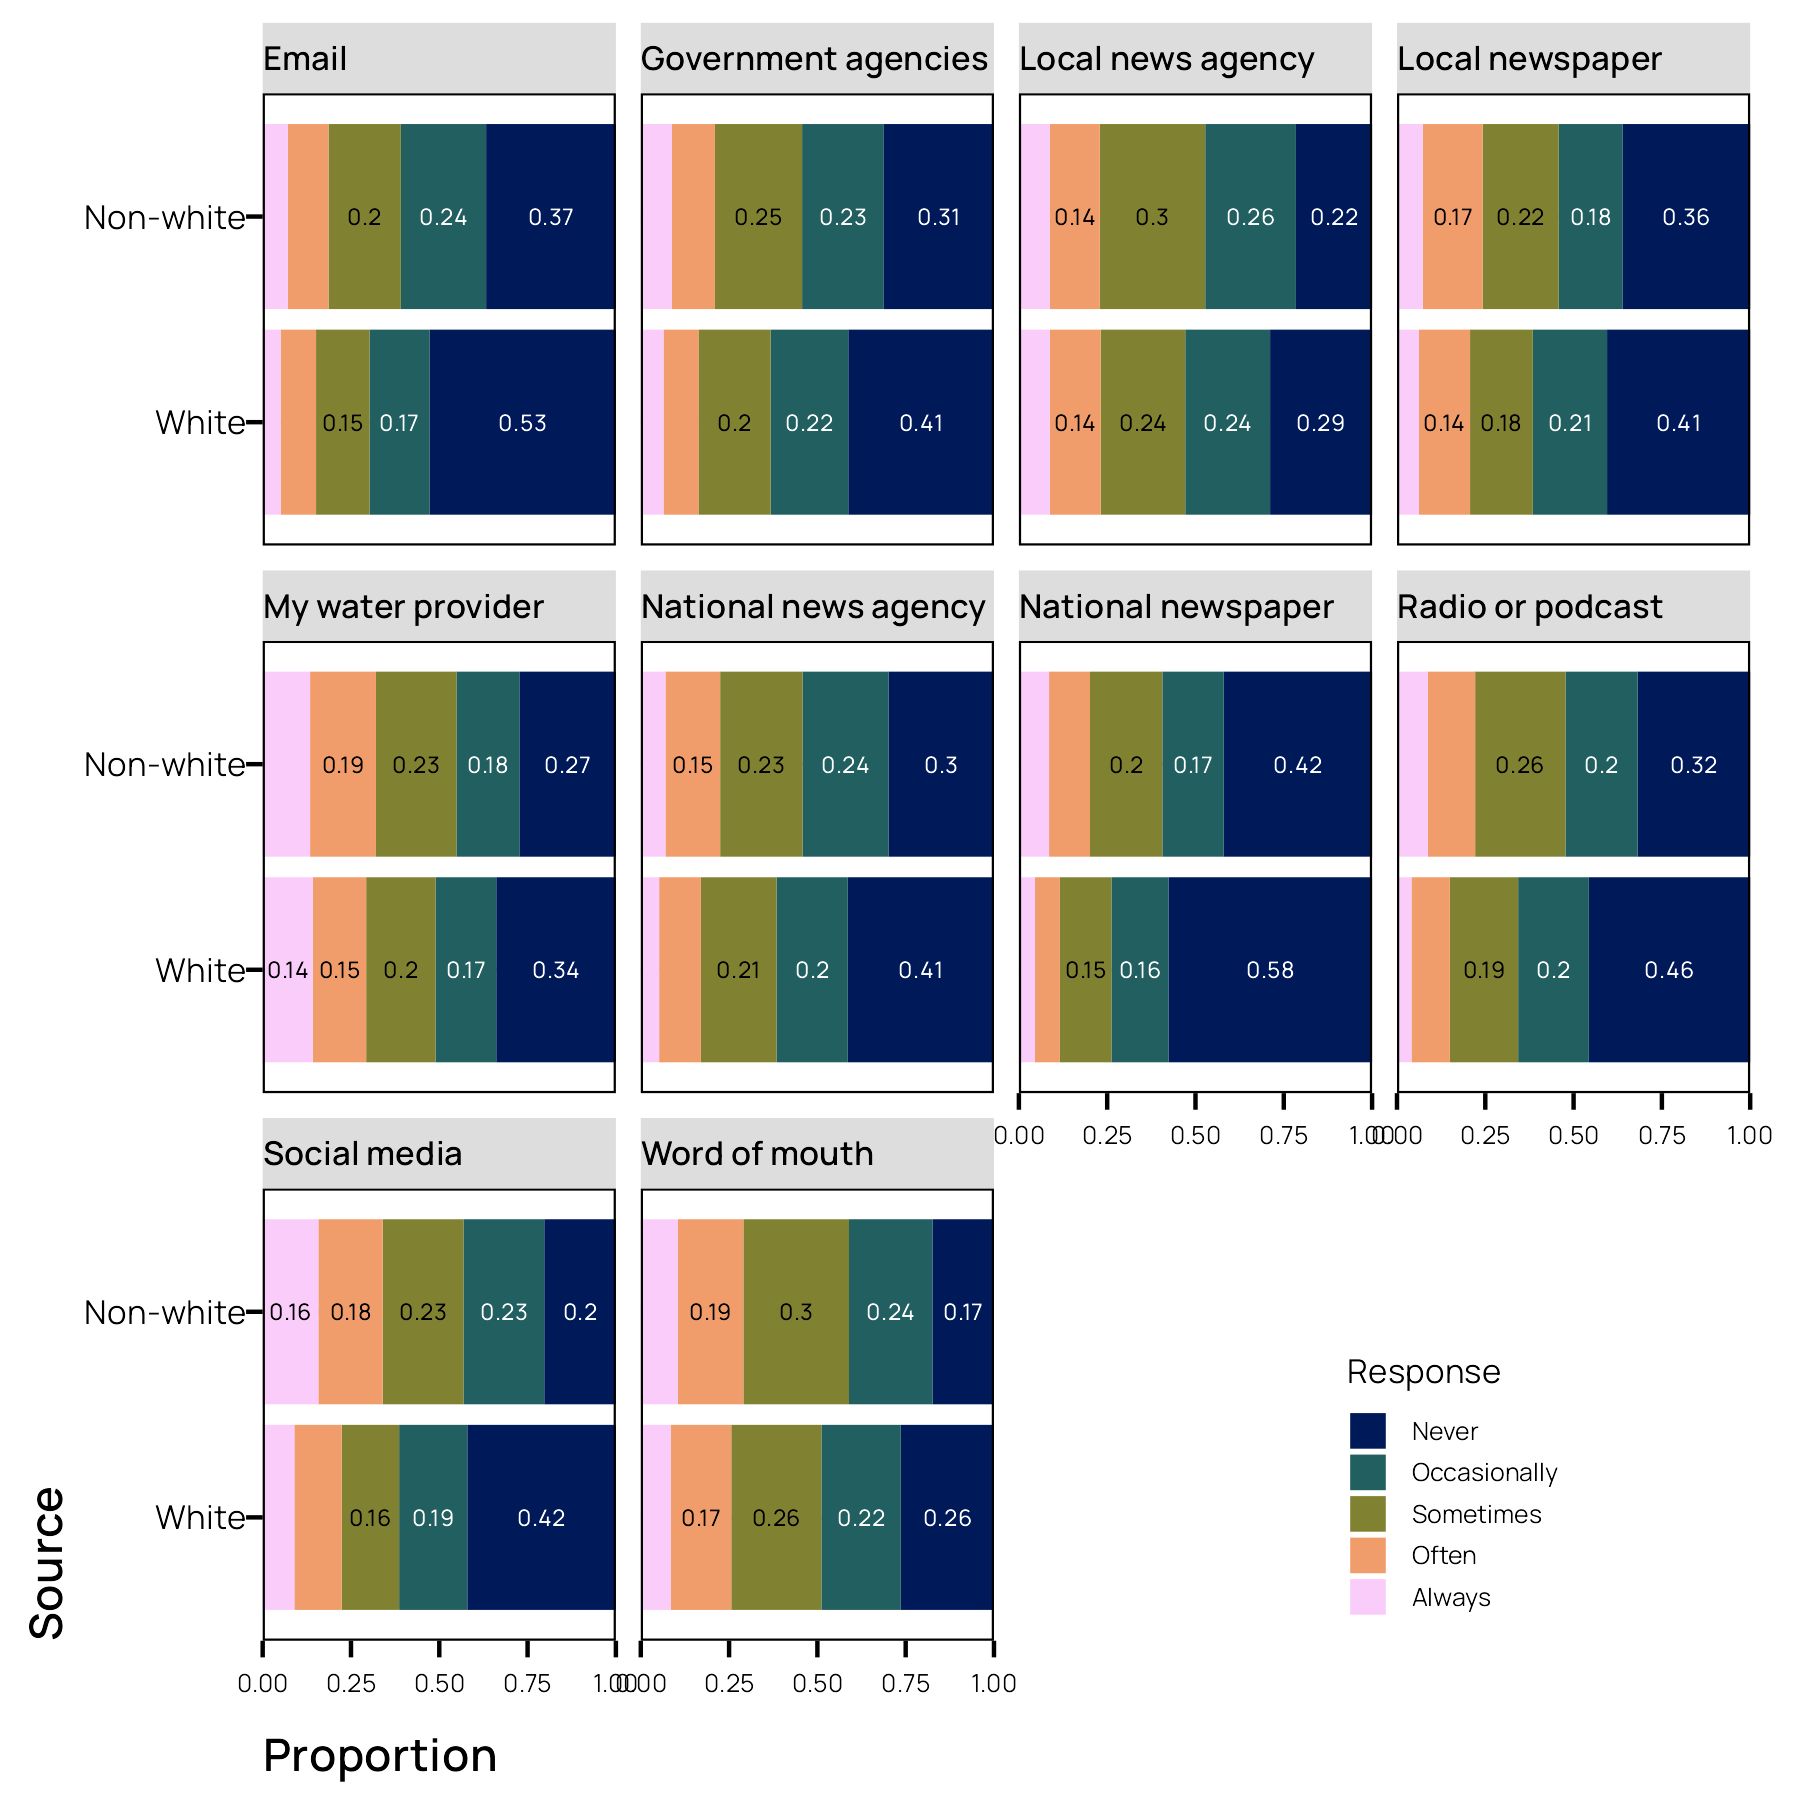
\includegraphics[width=1\textwidth,height=\textheight]{supplementary-materials_files/figure-pdf/fig-news-race-1.png}

}

\caption{\label{fig-news-race}Sources of drinking water quality
information by race/ethnicity.}

\end{figure}%

\begin{figure}

\centering{

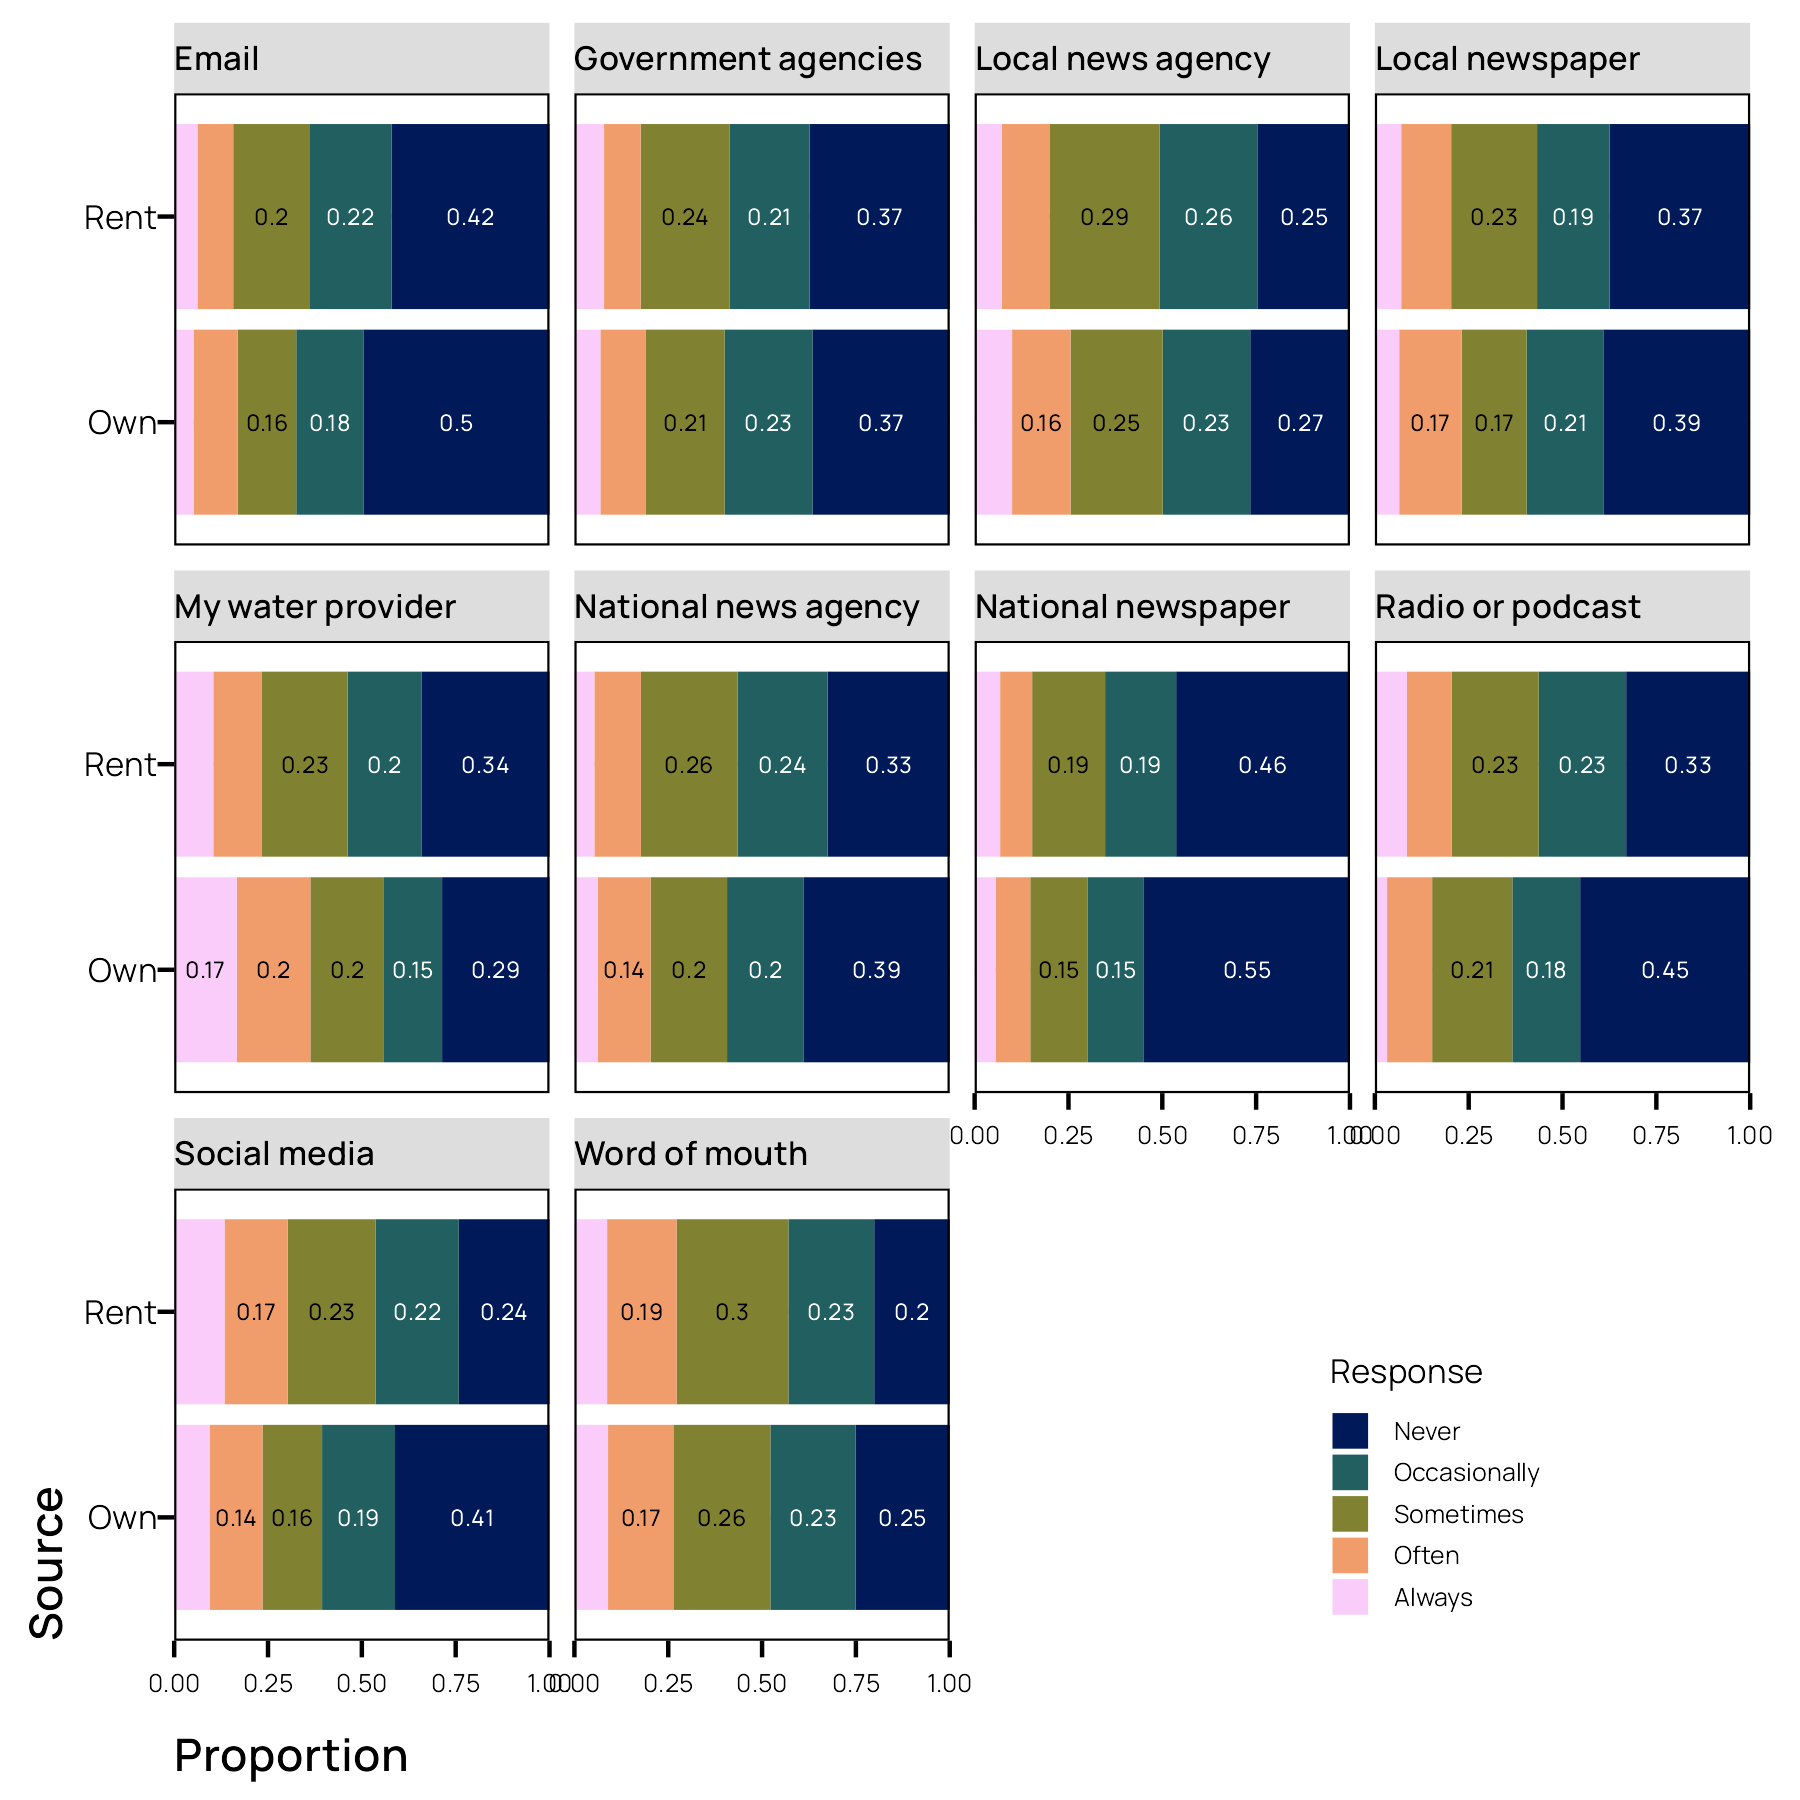
\includegraphics[width=1\textwidth,height=\textheight]{supplementary-materials_files/figure-pdf/fig-news-hownshp-1.png}

}

\caption{\label{fig-news-hownshp}Sources of drinking water quality
information by home ownership.}

\end{figure}%

\begin{figure}

\centering{

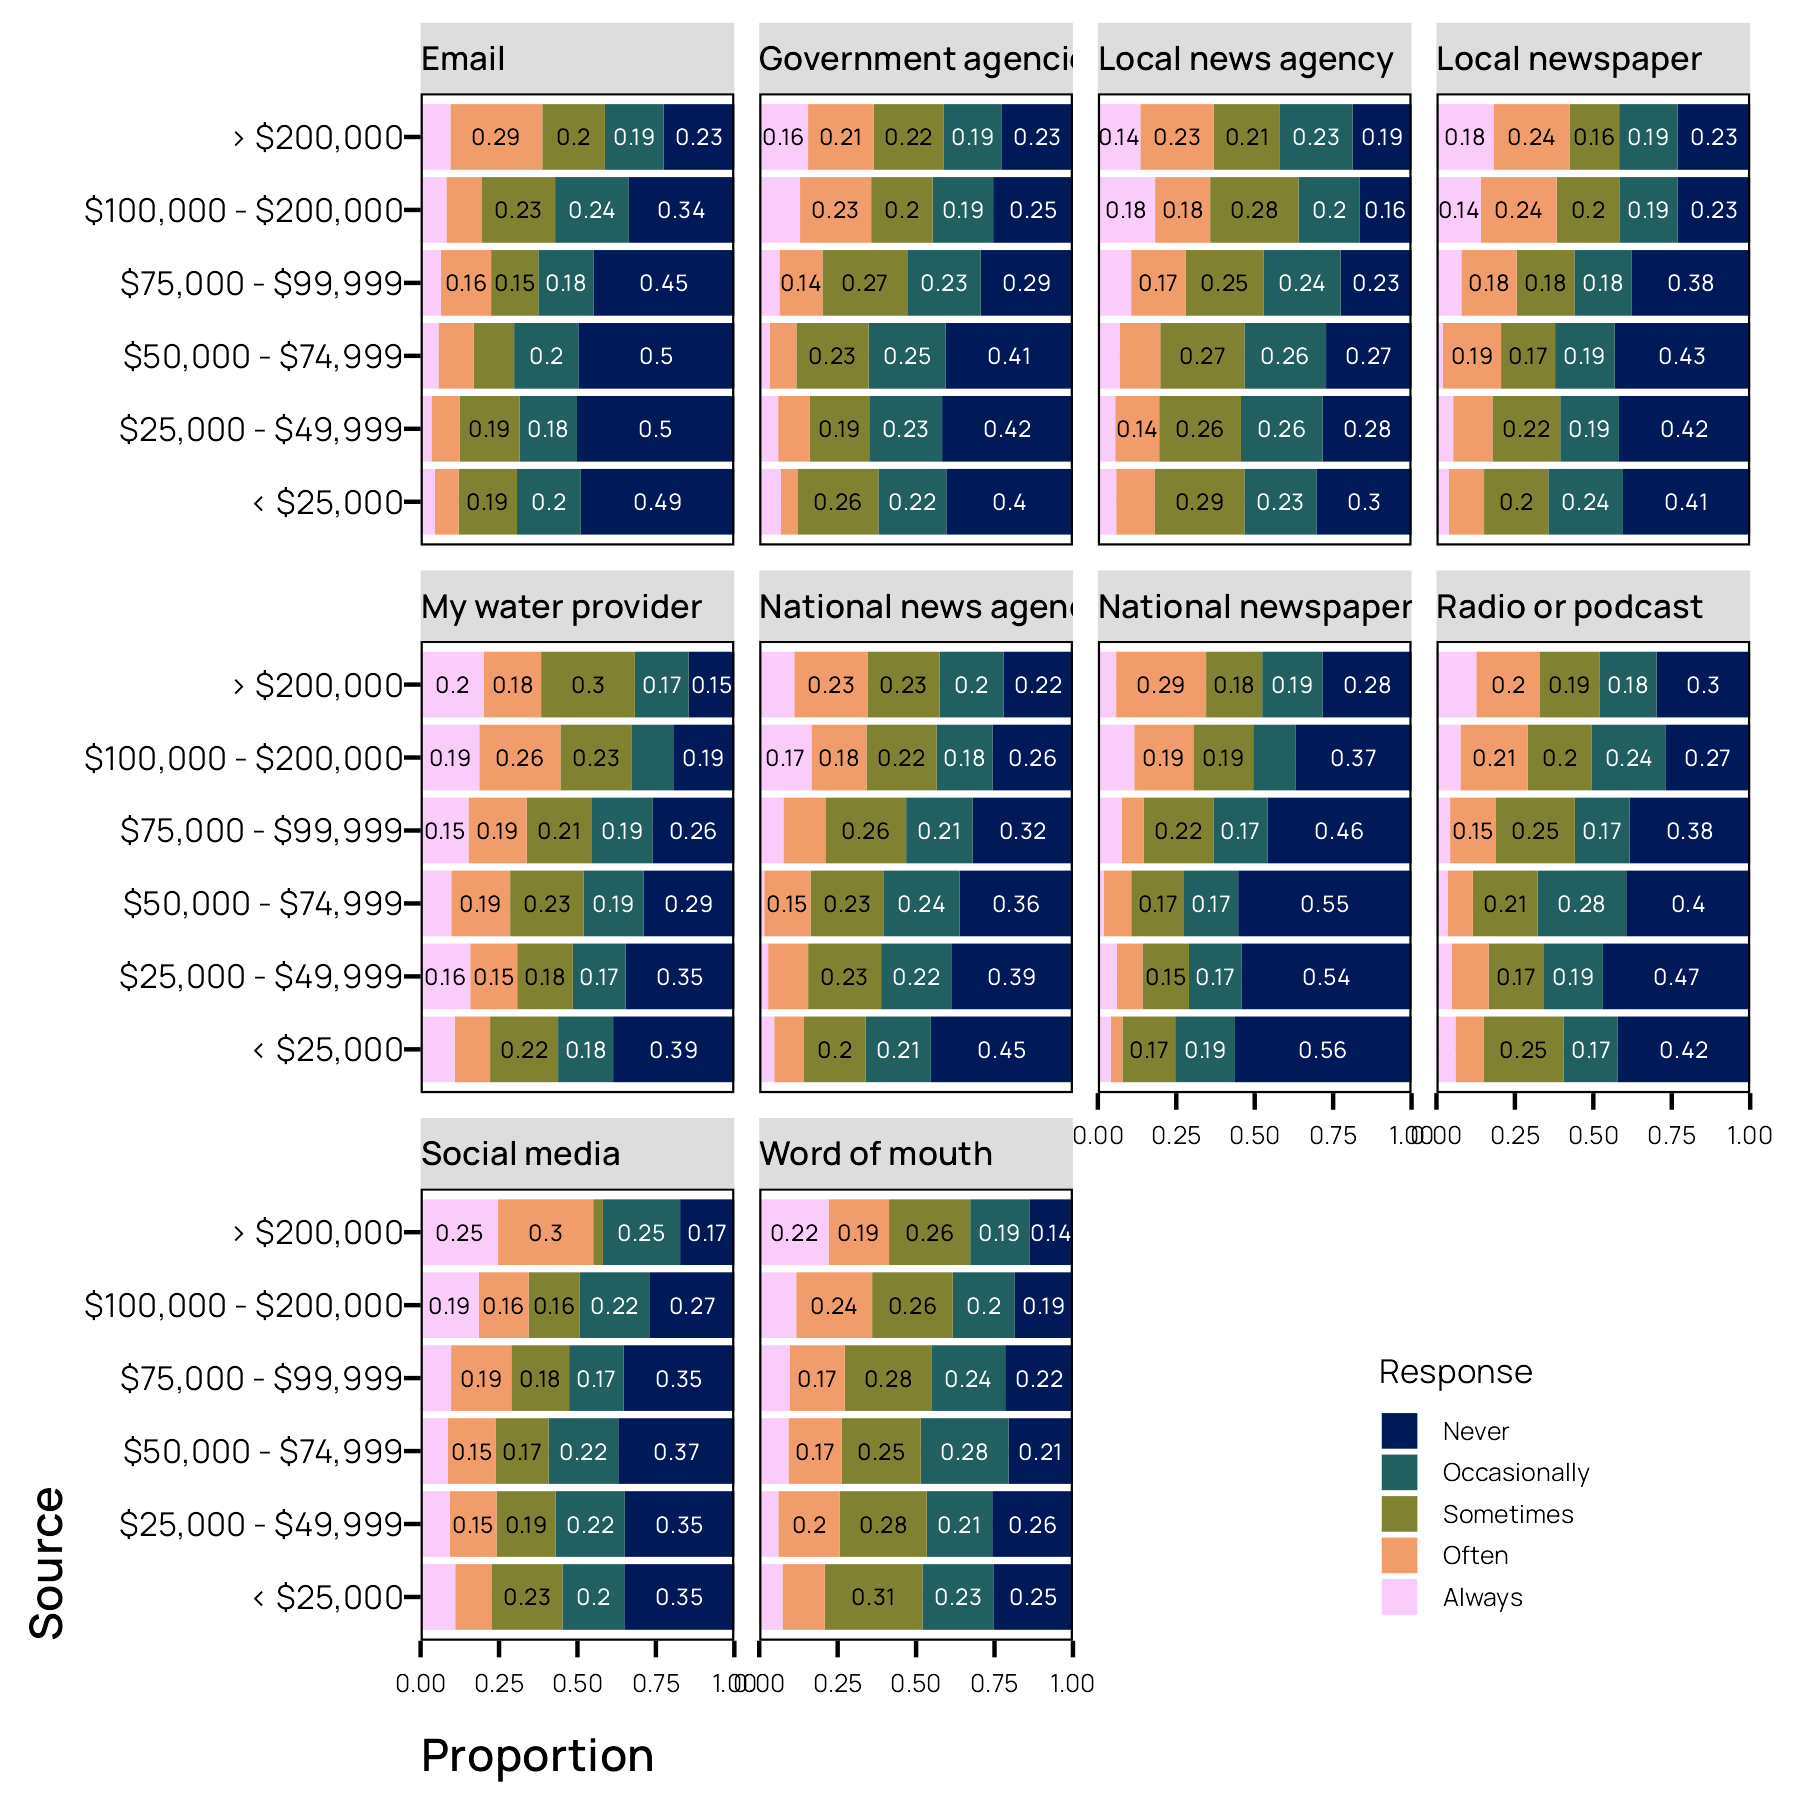
\includegraphics[width=1\textwidth,height=\textheight]{supplementary-materials_files/figure-pdf/fig-news-income-1.png}

}

\caption{\label{fig-news-income}Sources of drinking water quality
information by income.}

\end{figure}%

\begin{figure}

\centering{

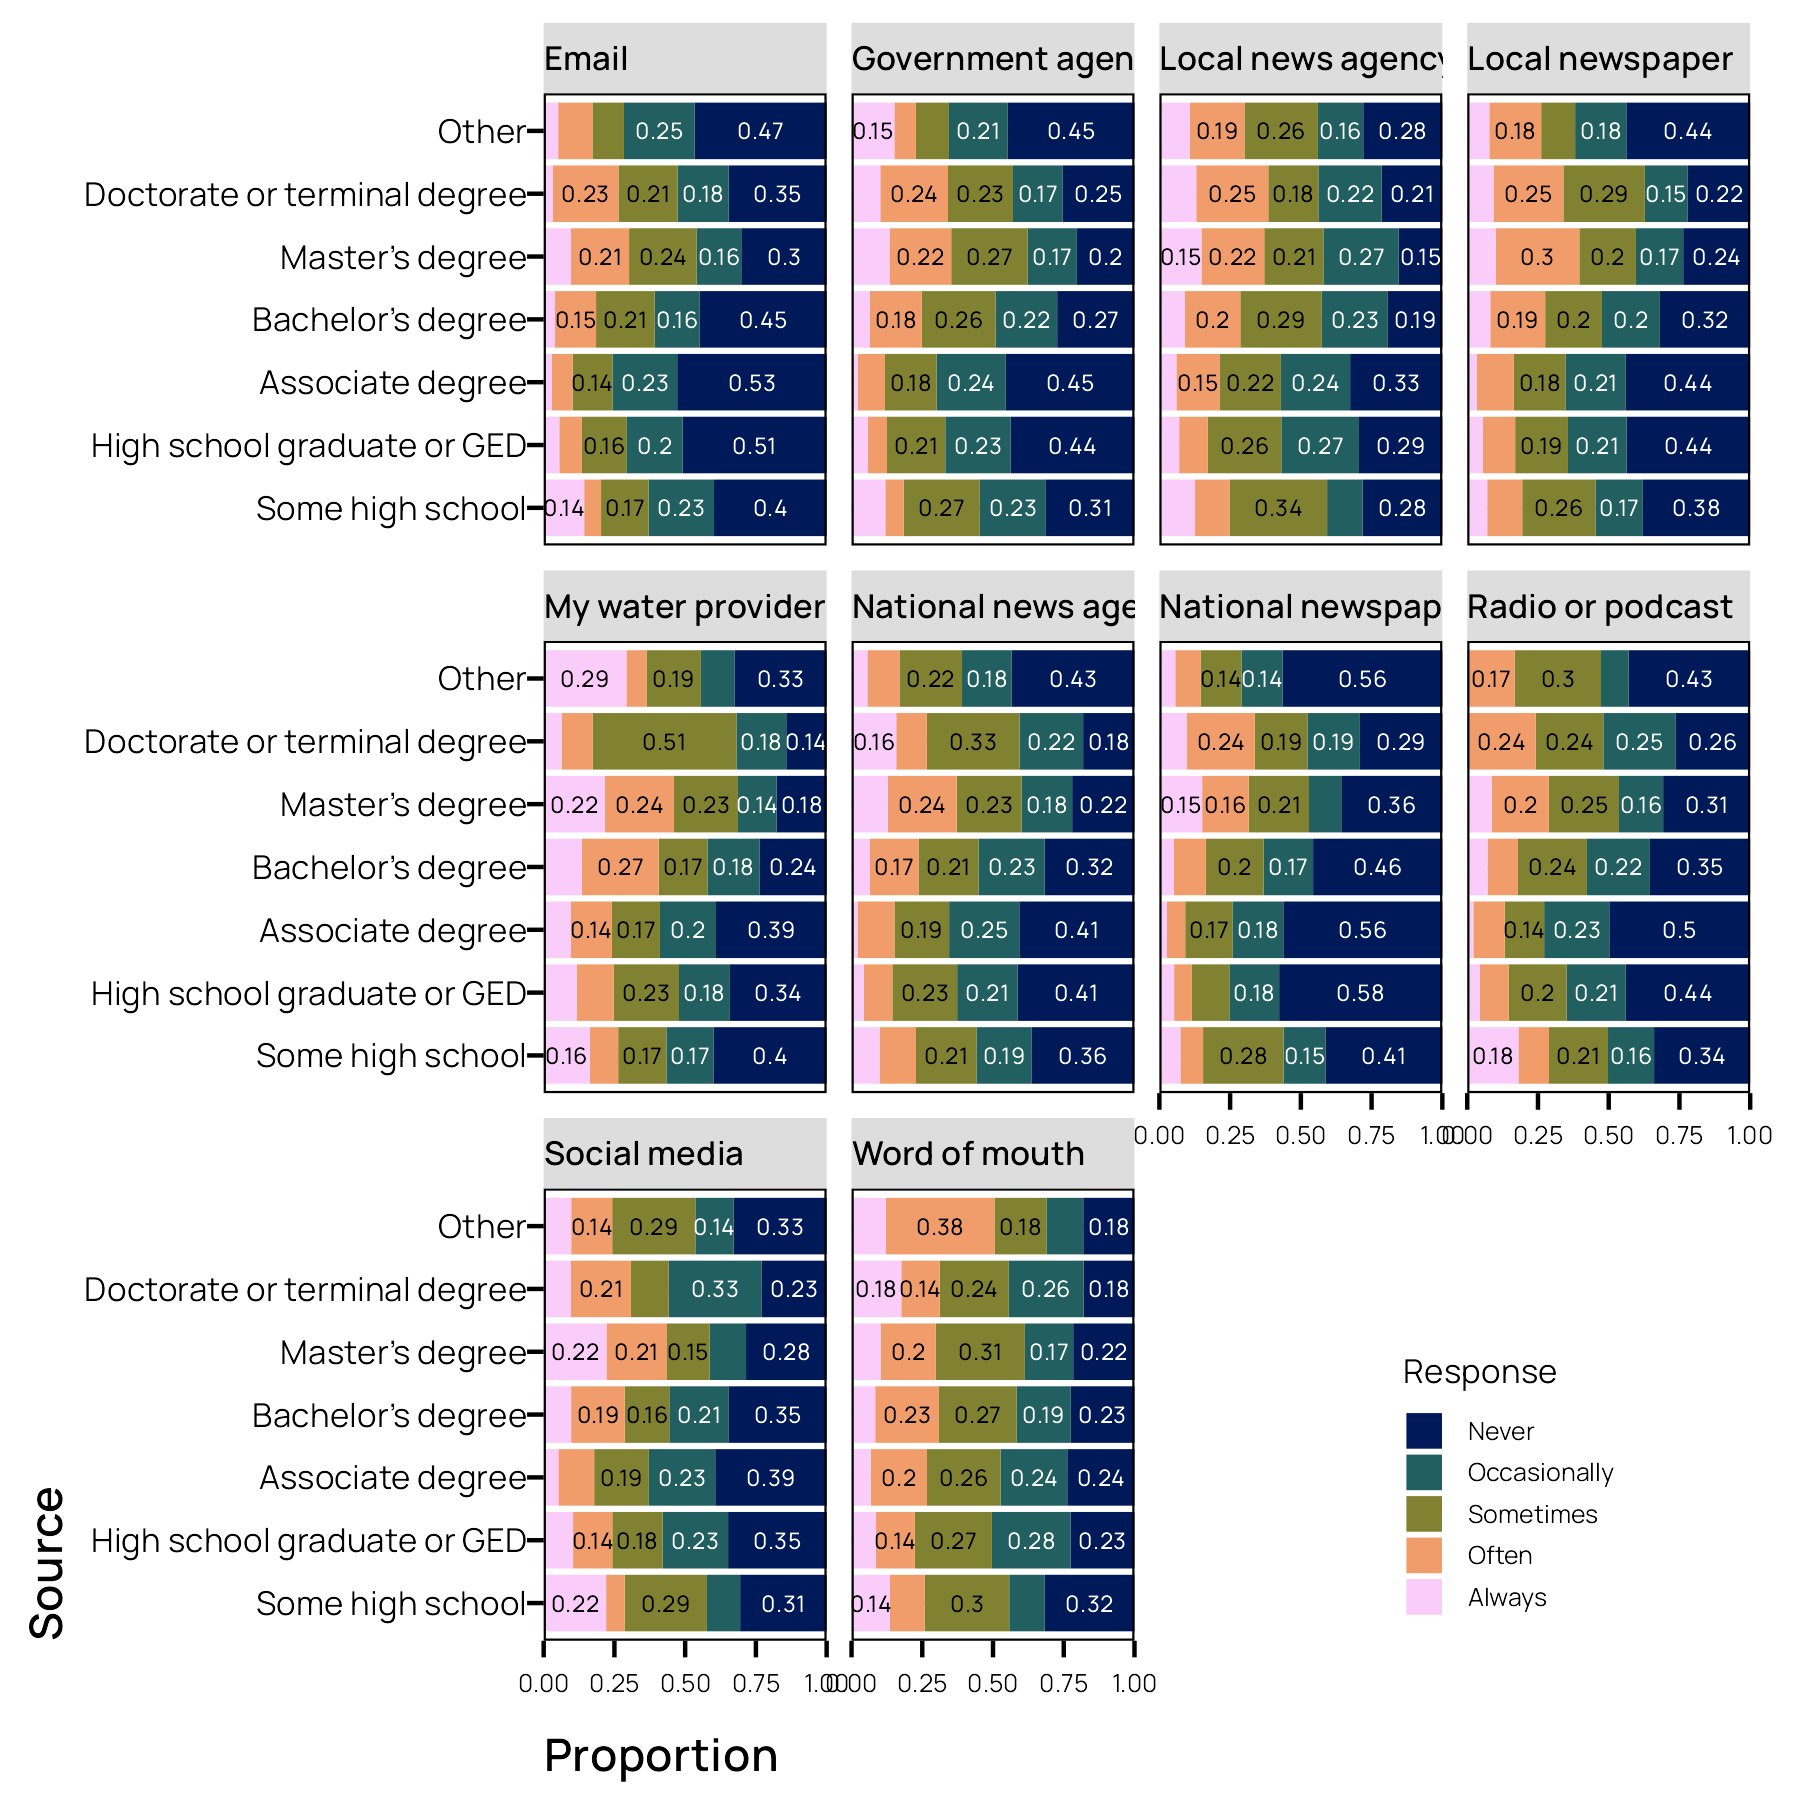
\includegraphics[width=1\textwidth,height=\textheight]{supplementary-materials_files/figure-pdf/fig-news-schl-1.png}

}

\caption{\label{fig-news-schl}Sources of drinking water quality
information by education.}

\end{figure}%

\newpage{}

\newgeometry{lmargin=1cm,rmargin=1cm}
\blandscape

\begin{longtblr}[         %% tabularray outer open
caption={},
caption={Results of multinomial logistic regression model for primary source of drinking water.  Odds-ratios are relative to unfiltered tap water. \label{tblr:m2}},
]                     %% tabularray outer close
{                     %% tabularray inner open
colspec={Q[]Q[]Q[]Q[]Q[]Q[]Q[]},
cell{1}{2}={c=3,}{halign=c,},
cell{1}{5}={c=3,}{halign=c,},
cell{4}{1}={c=7}{},cell{7}{1}={c=7}{},cell{13}{1}={c=7}{},cell{15}{1}={c=7}{},cell{22}{1}={c=7}{},cell{24}{1}={c=7}{},cell{30}{1}={c=7}{},cell{34}{1}={c=7}{},
cell{3}{1}={preto={\hspace{1em}}},
cell{5}{1}={preto={\hspace{1em}}},
cell{6}{1}={preto={\hspace{1em}}},
cell{8}{1}={preto={\hspace{1em}}},
cell{9}{1}={preto={\hspace{1em}}},
cell{10}{1}={preto={\hspace{1em}}},
cell{11}{1}={preto={\hspace{1em}}},
cell{12}{1}={preto={\hspace{1em}}},
cell{14}{1}={preto={\hspace{1em}}},
cell{16}{1}={preto={\hspace{1em}}},
cell{17}{1}={preto={\hspace{1em}}},
cell{18}{1}={preto={\hspace{1em}}},
cell{19}{1}={preto={\hspace{1em}}},
cell{20}{1}={preto={\hspace{1em}}},
cell{21}{1}={preto={\hspace{1em}}},
cell{23}{1}={preto={\hspace{1em}}},
cell{25}{1}={preto={\hspace{1em}}},
cell{26}{1}={preto={\hspace{1em}}},
cell{27}{1}={preto={\hspace{1em}}},
cell{28}{1}={preto={\hspace{1em}}},
cell{29}{1}={preto={\hspace{1em}}},
cell{31}{1}={preto={\hspace{1em}}},
cell{32}{1}={preto={\hspace{1em}}},
cell{33}{1}={preto={\hspace{1em}}},
cell{35}{1}={preto={\hspace{1em}}},
cell{36}{1}={preto={\hspace{1em}}},
rulesep={0pt}, rowsep={0pt}, colsep = {.5em}, vspan={default},
}                     %% tabularray inner close
\toprule
& Filtered tap water &  &  & Bottled water &  &  \\ \cmidrule[lr]{2-4}\cmidrule[lr]{5-7}
Variable & Odds-Ratio, [95\% CI] & t-statistic & p-value & Odds-Ratio, [95\% CI] & t-statistic & p-value \\ \midrule %% TinyTableHeader
(Intercept) & 0.7, [0.21, 2.31]   & -0.59 & 0.558 & 0.5, [0.16, 1.58]  & -1.18 & 0.240 \\
Sex/Gender &&&&&& \\
Female & 1.06, [0.73, 1.54]  &  0.32 & 0.752 & 1.49, [1.02, 2.17] &  2.08 & 0.038 \\
Other & 0.22, [0.01, 4.17]  & -1.01 & 0.311 & 0.51, [0.04, 6.17] & -0.53 & 0.595 \\
Age &&&&&& \\
25:34 & 0.95, [0.42, 2.13]  & -0.13 & 0.897 & 1.22, [0.53, 2.81] &  0.47 & 0.641 \\
35:44 & 0.52, [0.24, 1.14]  & -1.64 & 0.100 & 0.96, [0.43, 2.13] & -0.11 & 0.911 \\
45:54 & 0.29, [0.13, 0.64]  & -3.09 & 0.002 & 0.69, [0.32, 1.5]  & -0.94 & 0.348 \\
55:64 & 0.29, [0.13, 0.65]  & -3.02 & 0.002 & 0.58, [0.25, 1.33] & -1.28 & 0.201 \\
65+ & 0.28, [0.13, 0.62]  & -3.15 & 0.002 & 0.74, [0.33, 1.69] & -0.71 & 0.480 \\
Race/Ethnicity &&&&&& \\
Non-white & 1.17, [0.74, 1.85]  &  0.68 & 0.496 & 1.59, [1.01, 2.52] &  1.99 & 0.046 \\
Education &&&&&& \\
High school graduate or GED & 2.37, [0.93, 6.03]  &  1.82 & 0.069 & 1.08, [0.5, 2.37]  &  0.20 & 0.840 \\
Associate degree & 1.46, [0.54, 3.94]  &  0.75 & 0.451 & 0.7, [0.3, 1.64]   & -0.82 & 0.410 \\
Bachelor's degree & 4.31, [1.59, 11.66] &  2.88 & 0.004 & 1.24, [0.51, 3.01] &  0.47 & 0.642 \\
Master's degree & 3.06, [1.09, 8.59]  &  2.12 & 0.034 & 1.07, [0.41, 2.76] &  0.13 & 0.894 \\
Doctorate or terminal degree & 2.81, [0.72, 11]    &  1.48 & 0.138 & 0.63, [0.16, 2.5]  & -0.66 & 0.509 \\
Other & 1.23, [0.33, 4.56]  &  0.32 & 0.752 & 1.57, [0.53, 4.67] &  0.81 & 0.417 \\
Home Ownership &&&&&& \\
Rent & 1.28, [0.86, 1.91]  &  1.21 & 0.226 & 1.64, [1.07, 2.5]  &  2.29 & 0.022 \\
Income &&&&&& \\
\$25,000 - \$49,999 & 1.35, [0.79, 2.3]   &  1.10 & 0.271 & 1.22, [0.72, 2.07] &  0.75 & 0.455 \\
\$50,000 - \$74,999 & 2.2, [1.23, 3.93]   &  2.66 & 0.008 & 1.56, [0.86, 2.83] &  1.46 & 0.145 \\
\$75,000 - \$99,999 & 1.83, [0.96, 3.5]   &  1.82 & 0.068 & 1.66, [0.84, 3.27] &  1.46 & 0.145 \\
\$100,000 - \$200,000 & 1.52, [0.77, 3]     &  1.20 & 0.230 & 0.93, [0.45, 1.9]  & -0.20 & 0.838 \\
> \$200,000 & 2.73, [0.94, 7.97]  &  1.84 & 0.066 & 2.51, [0.78, 8.08] &  1.54 & 0.123 \\
Primary tap water supply &&&&&& \\
Public supply - rural water district & 1.37, [0.82, 2.28]  &  1.21 & 0.227 & 1.25, [0.74, 2.11] &  0.82 & 0.413 \\
Private supply - well, river, pond, rainwater & 0.83, [0.5, 1.39]   & -0.70 & 0.486 & 0.8, [0.47, 1.38]  & -0.79 & 0.427 \\
I don't know & 1.16, [0.6, 2.26]   &  0.44 & 0.663 & 1.6, [0.85, 3]     &  1.45 & 0.147 \\
Taste, odor, color issues &&&&&& \\
Yes & 1.07, [0.75, 1.52]  &  0.35 & 0.723 & 1.4, [0.96, 2.04]  &  1.75 & 0.081 \\
\bottomrule
\end{longtblr}

\elandscape
\restoregeometry

\newpage{}

\newgeometry{lmargin=1cm,rmargin=1cm}
\blandscape

\begin{longtblr}[         %% tabularray outer open
caption={},
caption = {Results of proportional odds-models on (1) water safety rating and (2) trust in water utilities. Model coefficients are displayed as odds-ratios relative to the reference level for each variable.\label{tblr:m13}},
]                     %% tabularray outer close
{                     %% tabularray inner open
colspec={Q[]Q[]Q[]Q[]Q[]Q[]Q[]},
cell{1}{2}={c=3,}{halign=c,},
cell{1}{5}={c=3,}{halign=c,},
cell{3}{1}={c=7}{},cell{7}{1}={c=7}{},cell{14}{1}={c=7}{},cell{17}{1}={c=7}{},cell{25}{1}={c=7}{},cell{28}{1}={c=7}{},cell{35}{1}={c=7}{},cell{40}{1}={c=7}{},
cell{4}{1}={preto={\hspace{1em}}},
cell{5}{1}={preto={\hspace{1em}}},
cell{6}{1}={preto={\hspace{1em}}},
cell{8}{1}={preto={\hspace{1em}}},
cell{9}{1}={preto={\hspace{1em}}},
cell{10}{1}={preto={\hspace{1em}}},
cell{11}{1}={preto={\hspace{1em}}},
cell{12}{1}={preto={\hspace{1em}}},
cell{13}{1}={preto={\hspace{1em}}},
cell{15}{1}={preto={\hspace{1em}}},
cell{16}{1}={preto={\hspace{1em}}},
cell{18}{1}={preto={\hspace{1em}}},
cell{19}{1}={preto={\hspace{1em}}},
cell{20}{1}={preto={\hspace{1em}}},
cell{21}{1}={preto={\hspace{1em}}},
cell{22}{1}={preto={\hspace{1em}}},
cell{23}{1}={preto={\hspace{1em}}},
cell{24}{1}={preto={\hspace{1em}}},
cell{26}{1}={preto={\hspace{1em}}},
cell{27}{1}={preto={\hspace{1em}}},
cell{29}{1}={preto={\hspace{1em}}},
cell{30}{1}={preto={\hspace{1em}}},
cell{31}{1}={preto={\hspace{1em}}},
cell{32}{1}={preto={\hspace{1em}}},
cell{33}{1}={preto={\hspace{1em}}},
cell{34}{1}={preto={\hspace{1em}}},
cell{36}{1}={preto={\hspace{1em}}},
cell{37}{1}={preto={\hspace{1em}}},
cell{38}{1}={preto={\hspace{1em}}},
cell{39}{1}={preto={\hspace{1em}}},
cell{41}{1}={preto={\hspace{1em}}},
cell{42}{1}={preto={\hspace{1em}}},
cell{43}{1}={preto={\hspace{1em}}},
column{1}={halign=l,},
column{2}={halign=c,},
column{3}={halign=c,},
column{4}={halign=c,},
column{5}={halign=c,},
column{6}={halign=c,},
column{7}={halign=c,},
row{1}={halign=c,},
rulesep={0pt}, rowsep={0pt}, colsep = {.5em}, vspan={default},
}                     %% tabularray inner close
\toprule
& Water safety rating &  &  & Trust in water utility &  &  \\ \cmidrule[lr]{2-4}\cmidrule[lr]{5-7}
& Odds-Ratio, [95\% CI] & t-stat & p-value & Odds-Ratio, [95\% CI] & t-stat & p-value \\ \midrule %% TinyTableHeader
Sex/Gender &&&&&& \\
Male & -                    &        &       & -                    &        &        \\
Female & 0.883 [0.683, 1.141] & -0.954 & 0.340 & 0.760 [0.593, 0.974] & -2.169 & 0.030  \\
Other & 0.190 [0.014, 2.563] & -1.253 & 0.210 & 0.127 [0.051, 0.311] & -4.505 & <0.001 \\
Age &&&&&& \\
18:24 & -                    &        &       & -                    &        &        \\
25:34 & 0.906 [0.550, 1.491] & -0.390 & 0.697 & 0.935 [0.586, 1.493] & -0.280 & 0.779  \\
35:44 & 0.730 [0.439, 1.215] & -1.213 & 0.226 & 0.793 [0.484, 1.300] & -0.920 & 0.358  \\
45:54 & 0.528 [0.301, 0.928] & -2.221 & 0.027 & 0.457 [0.276, 0.759] & -3.029 & 0.003  \\
55:64 & 0.849 [0.485, 1.486] & -0.574 & 0.566 & 0.720 [0.429, 1.211] & -1.239 & 0.216  \\
65+ & 0.708 [0.416, 1.205] & -1.273 & 0.203 & 1.142 [0.675, 1.933] & 0.497  & 0.620  \\
Race/Ethnicity &&&&&& \\
White & -                    &        &       & -                    &        &        \\
Non-white & 0.859 [0.642, 1.148] & -1.029 & 0.304 & 0.783 [0.575, 1.067] & -1.550 & 0.122  \\
Education &&&&&& \\
Some high school & -                    &        &       & -                    &        &        \\
High school graduate or GED & 1.920 [0.926, 3.980] & 1.756  & 0.079 & 1.243 [0.580, 2.664] & 0.560  & 0.576  \\
Associate degree & 1.715 [0.794, 3.702] & 1.376  & 0.169 & 1.025 [0.461, 2.282] & 0.061  & 0.951  \\
Bachelor's degree & 2.185 [1.019, 4.684] & 2.012  & 0.045 & 1.514 [0.681, 3.363] & 1.019  & 0.308  \\
Master's degree & 3.339 [1.487, 7.494] & 2.926  & 0.004 & 2.001 [0.881, 4.545] & 1.660  & 0.097  \\
Doctorate or terminal degree & 2.274 [0.757, 6.829] & 1.466  & 0.143 & 1.684 [0.685, 4.141] & 1.138  & 0.256  \\
Other & 1.814 [0.694, 4.738] & 1.217  & 0.224 & 0.951 [0.366, 2.472] & -0.103 & 0.918  \\
Homeownership &&&&&& \\
Own & -                    &        &       & -                    &        &        \\
Rent & 0.689 [0.527, 0.901] & -2.721 & 0.007 & 0.676 [0.513, 0.889] & -2.799 & 0.005  \\
Income &&&&&& \\
< \$25,000 & -                    &        &       & -                    &        &        \\
\$25,000 - \$49,999 & 0.790 [0.547, 1.141] & -1.259 & 0.209 & 1.187 [0.815, 1.728] & 0.895  & 0.371  \\
\$50,000 - \$74,999 & 0.864 [0.577, 1.294] & -0.710 & 0.478 & 1.075 [0.720, 1.605] & 0.354  & 0.723  \\
\$75,000 - \$99,999 & 0.701 [0.444, 1.107] & -1.526 & 0.127 & 0.901 [0.574, 1.416] & -0.451 & 0.652  \\
\$100,000 - \$200,000 & 1.529 [0.976, 2.396] & 1.855  & 0.064 & 1.502 [0.962, 2.344] & 1.793  & 0.073  \\
> \$200,000 & 0.872 [0.400, 1.898] & -0.346 & 0.729 & 1.823 [0.895, 3.710] & 1.657  & 0.098  \\
Primary tap water supply &&&&&& \\
Public supply - municipal & -                    &        &       & -                    &        &        \\
Public supply - rural water district & 1.070 [0.768, 1.490] & 0.400  & 0.689 & 0.808 [0.582, 1.124] & -1.268 & 0.205  \\
Private supply - well, river, pond, rainwater & 0.763 [0.547, 1.064] & -1.597 & 0.111 & 1.544 [1.098, 2.173] & 2.498  & 0.013  \\
I don't know & 0.882 [0.568, 1.368] & -0.563 & 0.574 & 0.992 [0.617, 1.594] & -0.034 & 0.973  \\
Taste, odor, color issues &&&&&& \\
No & -                    &        &       & -                    &        &        \\
Yes & 0.728 [0.568, 0.932] & -2.516 & 0.012 & 0.321 [0.248, 0.415] & -8.695 & <0.001 \\
\bottomrule
\end{longtblr}

\elandscape
\restoregeometry


\printbibliography[title=References]


\end{document}
